\documentclass[11pt]{article}
\usepackage[a4paper, total={6.5in, 9.5in}]{geometry}
\usepackage{graphicx}
\graphicspath{ {./images/output/} }
\usepackage{caption}
\usepackage[english]{babel}
\usepackage{titling}
\usepackage{float}
% \usepackage{amsmath}
% \usepackage{minted}
% \usepackage{multicol}
% \usepackage{array}
% \usepackage{setspace}
% \usepackage{placeins}

% \usepackage{lipsum}

\title{Experiment 1 \\
    \textbf{Study of ECG Signal Using Digital Electrocardiogram Device}}
\author{}
\date{}

\pagenumbering{gobble}
\begin{document}
\vspace*{\fill}
\begin{center}

    \emph{Heaven's Light is Our Guide} \\
    \textbf{Rajshahi University of Engineering and Technology} \\

    \begin{figure}[H]
        \centering
        
\includegraphics[scale=.34]{images/RUET_logo.png}
        \label{fig:ruet_logo}
    \end{figure}
    \vspace{5mm}

    \textbf{Course Code}\\
    ECE 4144\\
    \vspace{3mm}
    \textbf{Course Title}\\
    Biomedical Engineering Sessional

    \vspace{5mm}
    \textbf{Experiment Date:} {August 06, 2025},\\
    \textbf{Submission Date:} {August 13, 2025}\\

    \vspace{5mm}
    \textbf{Lab Report 3: \\
        Experimental Observation of Various Features of an ECG
        Signal Collected from PhysioNet Public Dataset}

    \vspace{15mm}

    \begin{tabular}{c|c}
        \textbf{Submitted to} & \textbf{Submitted by} \\
        Md Mayenul Islam      & Md. Tajim An Noor     \\
        Assistant Professor   & Roll: 2010025         \\
        Dept of EEE, Ruet     &                       \\
    \end{tabular}

\end{center}
\vspace*{\fill}


\pagebreak
\maketitle

\section*{Objectives}
\begin{itemize}
    \item Acquire and examine human ECG signals utilizing a digital electrocardiograph with 10 leads.
    \item Detect and distinguish ECG waveform features, including the P wave, QRS complex, and T wave.
    \item Comprehend the positioning and importance of limb and chest leads for interpreting ECG results.
\end{itemize}

\section*{Theory}
An electrocardiogram (ECG) records the heart’s electrical signals using electrodes placed on the skin. In clinical practice, a typical ECG setup employs 10 electrodes—4 on the limbs and 6 on the chest—to generate 12 distinct leads. These include 3 standard limb leads (I, II, III), 3 augmented limb leads (aVR, aVL, aVF), and 6 precordial (chest) leads (V1–V6). Each lead offers a different perspective on the heart’s electrical activity, aiding in comprehensive cardiac assessment. By analyzing changes in the P wave, QRS complex, and T wave across these leads, clinicians can detect irregularities such as arrhythmias, heart attacks, and other cardiac disorders.

\subsection*{ECG Lead Types and Electrode Placement}
\begin{itemize}
    \item \textbf{Lead I} (Limb; Right Arm): LA - RA
    \item \textbf{Lead II} (Limb; Left Arm): LL - RA
    \item \textbf{Lead III} (Limb; Left Leg): LL - LA
    \item \textbf{Lead IV} (Limb; Right Leg): Ground
    \item \textbf{aVR} (Augmented): RA - (LA + LL)/2
    \item \textbf{aVL} (Augmented): LA - (RA + LL)/2
    \item \textbf{aVF} (Augmented): LL - (RA + LA)/2
    \item \textbf{V1} (Chest): 4th intercostal space, right sternal border
    \item \textbf{V2} (Chest): 4th intercostal space, left sternal border
    \item \textbf{V3} (Chest): Between V2 and V4
    \item \textbf{V4} (Chest): 5th intercostal space, midclavicular line
    \item \textbf{V5} (Chest): Same level as V4, anterior axillary line
    \item \textbf{V6} (Chest): Same level as V4, midaxillary line
\end{itemize}

\section*{Required Equipment}
\begin{itemize}
    \item 10-lead Digital Electrocardiograph (HP-1300plus)
    \item ECG lead wires and disposable electrodes
    \item Volunteer human subject
    \item ECG paper or digital display for signal observation
\end{itemize}


\section*{Experimental Observation}
\begin{itemize}
    \item The volunteer was asked to relax and remain still in a supine position to minimize motion artifacts.
    \item Standard electrode placement was followed: four electrodes were attached to the limbs and six to the chest at designated anatomical locations.
    \item The digital ECG system successfully recorded signals from all twelve leads, providing clear and consistent waveforms.
    \item Lead II produced the most prominent and stable trace, which was used to determine the subject’s heart rate.
    \item The characteristic ECG features—P wave, QRS complex, and T wave—were easily identified in the recordings.
    \item The subject’s ECG showed normal sinus rhythm, with no evidence of arrhythmias or abnormal patterns.
\end{itemize}

\begin{figure}[H]
    \centering
    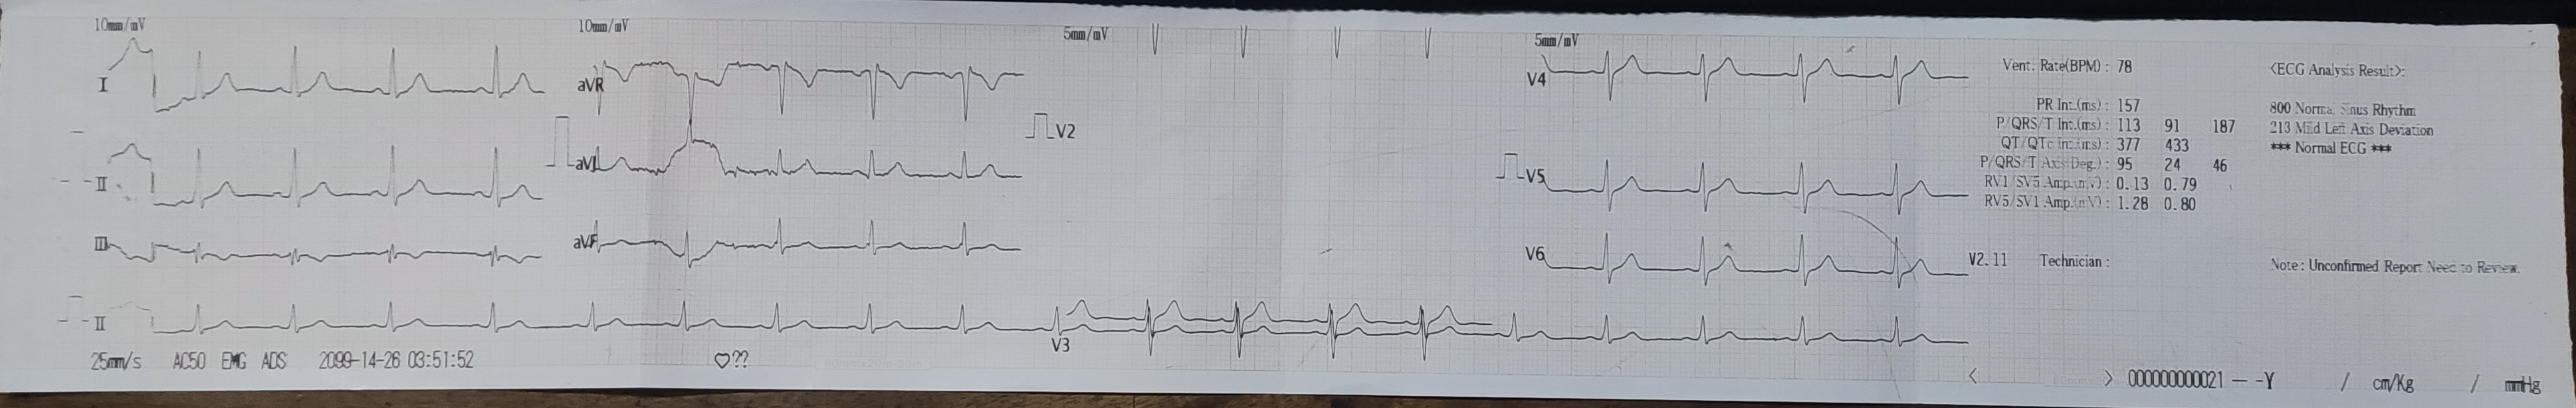
\includegraphics[width=1\textwidth]{1.jpg}
    \caption{ECG}
\end{figure}

\section*{Discussion}
\addcontentsline{toc}{section}{Discussion}
Using the HP-1300plus digital ECG device, twelve standard leads were recorded with reliable signal quality. The device’s IEC60601-1 safety compliance ensured safe use. Proper electrode placement was crucial for accurate waveforms, with Lead II providing the clearest signal for heart rate measurement. This experiment enhanced understanding of cardiac conduction and the clinical value of different ECG leads.

\bibliographystyle{IEEEtran}
\renewcommand{\bibname}{References}
\addcontentsline{toc}{section}{References}
\bibliography{ref}

\end{document}
